\documentclass{alex_hü}

\name{Alexander Helbok}
\course{PS Physik}
\hwnumber{7}
\usepackage{biblatex}

\begin{document}
\renewcommand{\labelenumi}{\alph{enumi})}


\begin{mybox}{Wellenfunktion und Aufenthaltswahrscheinlichkeit eines Teilchens}
	\centering \(  \Psi(x) = \begin{cases}
		2 \quad &\text{für } 0 \leq x \leq 1 \\
		1 \quad &\text{für }  1 \le x \le 2 \\
		-2 \quad &\text{für }  2 \leq x \leq 3
	\end{cases} \)
	\tcblower
	\begin{enumerate}
		\item The probability of finding the particle is the lowest in sector \RN{2}
	\tcbline
		\item the unit of \( \psi(x) \) is \( \unit{\sqrt{m}} \) and the unit of \( x \) is meter \( \unit{m} \)
	\tcbline
		\item \(  \)
		The normalization condition states that \\
		\begin{flalign*}
			&\uint[-\infty, \infty]{\abs{A\psi(x)}^2}{x} = 1 &&
		\end{flalign*}
		In our case \\
		\begin{flalign*}
			\uint[-\infty, \infty]{\abs{A\psi(x)}^2}{x} &= A^2 \left[ \uint[0, 1]{1}{x} + \uint[1, 2]{4}{x} + \uint[2, 3]{4}{x} \right] = 9A^2 \overset{!}{=} 1 &&
		\end{flalign*}
		\( \Rightarrow A = \tfrac{1}{3} \)
	\tcbline
		\item \(  \)
		\begin{flalign*}
			P &= \uint[2, 3]{\frac{4}{9}}{x} = \dl{\frac{4}{9}} &&
		\end{flalign*}
	\tcbline
		\item \(  \)
		\begin{flalign*}
			P &= \uint[2, 3]{\abs{\tfrac{2}{3} \expo[\pi/6][\iu]}^2}{x} = \uint[2, 3]{\frac{4}{9}}{x} = \dl{\frac{4}{9}} &&
		\end{flalign*}
	\end{enumerate}
\end{mybox}

\begin{mybox}{Teilchen im asymmetrischen Potentialtopf}
	\centering \( V(x) = \begin{cases}
		\infty \quad &\text{für } x \leq 0 \\
		-V_0 \quad &\text{für }  0 \le x \le a \\
		0 \quad &\text{für }  a \leq x
	\end{cases} \)
	\tcblower
	\begin{enumerate}
		\item \( -\tfrac{\hbar^2}{2m}\pdv[2]{\psi(x)}{x} + E_{\text{pot}} \psi(x) = E \psi(x) \)
		\begin{flalign*}
			\psi_1(x) &= 0 &&
		\end{flalign*}
	\tcbline
		\item \(  \)\\
		\underline{For \RN{2}:} \( \psi_{\text{\RN{2}}}(x) = A\sin(kx) + B\cos(kx)  \) \\[2ex]
		\underline{For \RN{3}:} \( \psi_{\text{\RN{3}}}(x) = C\expo[-][\kappa x] + D\expo[\kappa x]  \)\\[2ex]
		\underline{Boundary conditions:}
		\begin{flalign*}
			\psi_{\text{\RN{2}}}(x=0) &= 0 &&\\
			\psi_{\text{\RN{2}}}(x=a) &= \psi_{\text{\RN{3}}}(x=a) &&\\
			\dv{}{x} \psi_{\text{\RN{2}}}(x=0) &= 0 &&\\
			\dv{}{x} 	\psi_{\text{\RN{2}}}(x=a) &= \dv{}{x} \psi_{\text{\RN{3}}}(x=a) &&
		\end{flalign*}
	\tcbline
		\item \(  \)
		\begin{flalign*}
			k &= \pm \frac{\sqrt{2Em}}{\hbar} &&\\
			\kappa &= \pm \frac{\sqrt{2m(V_0-E)}}{\hbar} &&
		\end{flalign*}
	\tcbline
		\item \(  \)
%		\begin{flalign*}
		%			
%		\end{flalign*}
	\tcbline
		\item \(  \)
%		\begin{flalign*}
		%			
%		\end{flalign*}
	\tcbline
		\item \(  \)
%		\begin{flalign*}
		%			
%		\end{flalign*}
\tcbline
		\item \(  \)
%		\begin{flalign*}
	%			
	%		\end{flalign*}
	\end{enumerate}
\end{mybox}

\begin{mybox}{Teilchen an einem Potentialabfall}
	\centering \( V(x) = \begin{cases}
		V_0 \quad &\text{für } x \leq 0 \\
		0 \quad &\text{für }  x > 0 \\
	\end{cases} \)
	\tcblower
	\begin{enumerate}
		\item \(  \)
		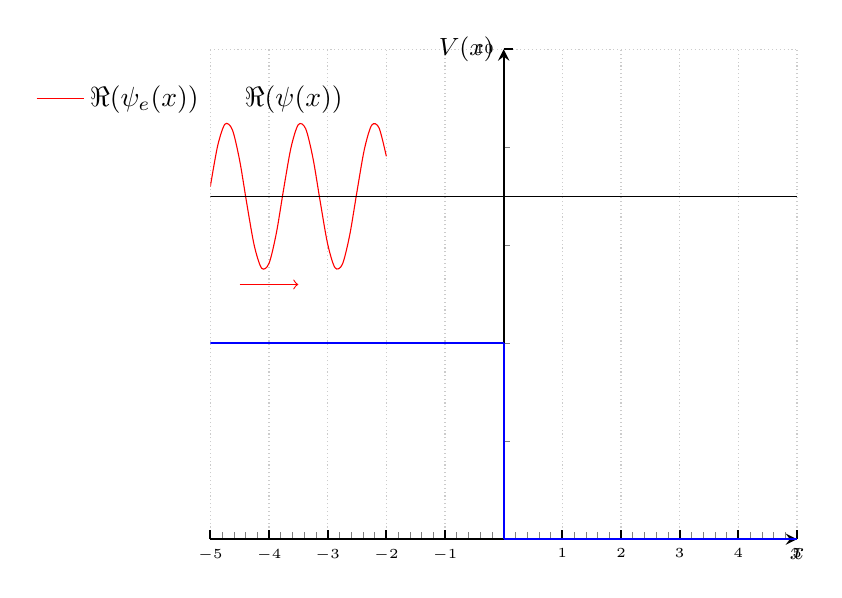
\begin{tikzpicture}
			\begin{axis}[
				every minor tick/.append style={minor tick length=0.085cm},
				every major tick/.append style={major tick length=0.12cm,thick,black},
				trig format plots=rad,
				width=257pt,
				height=222pt,
				axis lines=center,
				axis line style={thick},
				tick align=outside,
				xmin=-5,xmax=5,ymin=0,ymax=10,
				ticklabel style = {font=\tiny},
				tick align=inside,
				xlabel style={font=\small,below},
				ylabel style={font=\small,left},
				xtick distance=1,
				minor tick num=4,
				ytick distance=10,
				xlabel=$x$,
				ylabel=$V(x)$,
				grid=major,
				grid style={thin,densely dotted,black!20},
				legend columns=3,
				legend style={fill=none, draw=none, at={(axis description cs:0.25,0.9)},anchor=east}],
				\addplot [domain=-5:-2,smooth, red] {1.5*sin(5*x)+7};
				\draw [->, red] (-4.5, 5.2) -- (-3.5, 5.2);
				\addplot [domain=-5:0, blue, thick] {4};
				\addplot [domain=0:5, blue, thick] {0};
				\draw [blue, thick] (0,4) -- (0,0);
				\addplot [black] {7};
				\legend{$\Re(\psi_{\text{e}}(x))$ ~~~ $\Re(\psi(x))$}
			\end{axis}
		\end{tikzpicture}
	\tcbline
		\item \(  \)
		\begin{flalign*}
			\psi_{\text{t}}(x=0) &= \psi_{\text{e}}(x=0) + \psi_{\text{r}}(x=0) &&\\
			\dv{}{x} \psi_{\text{t}}(x=0) &= \dv{}{x} \left( \psi_{\text{e}}(x=0) + \psi_{\text{r}}(x=0)\right) &&
		\end{flalign*}
	\tcbline
		\item \(  \)
%		\begin{flalign*}
		%			
%		\end{flalign*}
	\tcbline
		\item \(  \)
%		\begin{flalign*}
	%			
%		\end{flalign*}
	\tcbline
		\item \(  \)
%		\begin{flalign*}
	%			
%		\end{flalign*}
	\tcbline
		\item \(  \)
%		\begin{flalign*}
	%			
%		\end{flalign*}
	\end{enumerate}
\end{mybox}


\end{document}